\documentclass{standalone}
\usepackage{tikz}
\usetikzlibrary{patterns, positioning}

\begin{document}
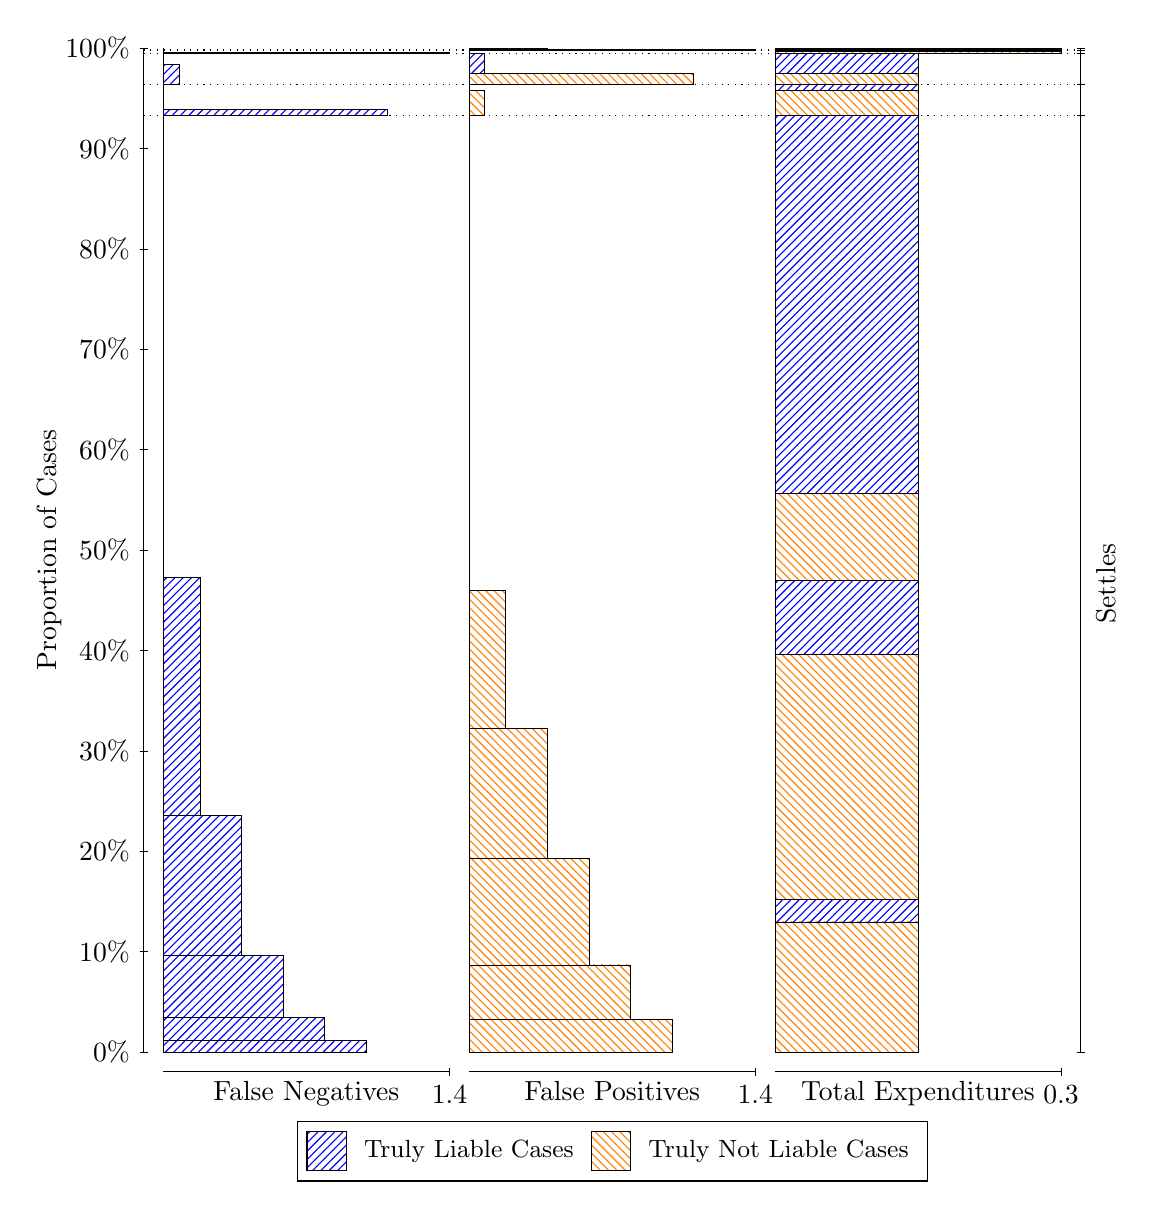
\begin{tikzpicture}
\draw[black, very thin] (1.5,1.75) -- (1.5,14.5);
\node[rotate=90, anchor=center] at (0.3, 8.125) {Proportion of Cases};
\draw[black, very thin] (1.45,1.75) -- (1.55,1.75);
\node[anchor=east] at (1.45, 1.75) {0\%};
\draw[black, very thin] (1.45,3.025) -- (1.55,3.025);
\node[anchor=east] at (1.45, 3.025) {10\%};
\draw[black, very thin] (1.45,4.3) -- (1.55,4.3);
\node[anchor=east] at (1.45, 4.3) {20\%};
\draw[black, very thin] (1.45,5.575) -- (1.55,5.575);
\node[anchor=east] at (1.45, 5.575) {30\%};
\draw[black, very thin] (1.45,6.85) -- (1.55,6.85);
\node[anchor=east] at (1.45, 6.85) {40\%};
\draw[black, very thin] (1.45,8.125) -- (1.55,8.125);
\node[anchor=east] at (1.45, 8.125) {50\%};
\draw[black, very thin] (1.45,9.4) -- (1.55,9.4);
\node[anchor=east] at (1.45, 9.4) {60\%};
\draw[black, very thin] (1.45,10.675) -- (1.55,10.675);
\node[anchor=east] at (1.45, 10.675) {70\%};
\draw[black, very thin] (1.45,11.95) -- (1.55,11.95);
\node[anchor=east] at (1.45, 11.95) {80\%};
\draw[black, very thin] (1.45,13.225) -- (1.55,13.225);
\node[anchor=east] at (1.45, 13.225) {90\%};
\draw[black, very thin] (1.45,14.5) -- (1.55,14.5);
\node[anchor=east] at (1.45, 14.5) {100\%};

\draw[black, very thin] (13.4,1.75) -- (13.4,14.5);
\draw[black, very thin] (13.35,1.75) -- (13.45,1.75);
\node[anchor=west] at (13.35, 1.75) {};
\draw[black, very thin] (13.35,13.642) -- (13.45,13.642);
\node[anchor=west] at (13.35, 13.642) {};
\draw[black, very thin] (13.35,14.041) -- (13.45,14.041);
\node[anchor=west] at (13.35, 14.041) {};
\draw[black, very thin] (13.35,14.43) -- (13.45,14.43);
\node[anchor=west] at (13.35, 14.43) {};
\draw[black, very thin] (13.35,14.475) -- (13.45,14.475);
\node[anchor=west] at (13.35, 14.475) {};
\draw[black, very thin] (13.35,14.5) -- (13.45,14.5);
\node[anchor=west] at (13.35, 14.5) {};

\draw[black, very thin, pattern color=blue, pattern=north east lines] (1.75,1.75) rectangle (4.3264,1.8999);
\draw[black, very thin, pattern color=blue, pattern=north east lines] (1.75,1.8999) rectangle (3.7979,2.1891);
\draw[black, very thin, pattern color=blue, pattern=north east lines] (1.75,2.1891) rectangle (3.2694,2.9754);
\draw[black, very thin, pattern color=blue, pattern=north east lines] (1.75,2.9754) rectangle (2.7409,4.7514);
\draw[black, very thin, pattern color=blue, pattern=north east lines] (1.75,4.7514) rectangle (2.2124,7.7762);
\draw[black, very thin, pattern color=orange, pattern=north west lines] (1.75,7.7762) rectangle (1.75,13.642);
\draw[black, very thin, pattern color=blue, pattern=north east lines] (1.75,13.642) rectangle (4.5906,13.717);
\draw[black, very thin, pattern color=orange, pattern=north west lines] (1.75,13.717) rectangle (1.75,14.041);
\draw[black, very thin, pattern color=blue, pattern=north east lines] (1.75,14.041) rectangle (1.9482,14.29);
\draw[black, very thin, pattern color=orange, pattern=north west lines] (1.75,14.29) rectangle (1.75,14.43);
\draw[black, very thin, pattern color=blue, pattern=north east lines] (1.75,14.43) rectangle (5.3833,14.442);
\draw[black, very thin, pattern color=orange, pattern=north west lines] (1.75,14.442) rectangle (1.75,14.475);
\draw[black, very thin, pattern color=orange, pattern=north west lines] (1.75,14.475) rectangle (1.75,14.487);
\draw[black, very thin, pattern color=blue, pattern=north east lines] (1.75,14.487) rectangle (1.75,14.5);
\draw[black, very thin, pattern color=orange, pattern=north west lines] (5.6333,1.75) rectangle (8.2097,2.167);
\draw[black, very thin, pattern color=orange, pattern=north west lines] (5.6333,2.167) rectangle (7.6812,2.8562);
\draw[black, very thin, pattern color=orange, pattern=north west lines] (5.6333,2.8562) rectangle (7.1527,4.2088);
\draw[black, very thin, pattern color=orange, pattern=north west lines] (5.6333,4.2088) rectangle (6.6242,5.8618);
\draw[black, very thin, pattern color=orange, pattern=north west lines] (5.6333,5.8618) rectangle (6.0958,7.6161);
\draw[black, very thin, pattern color=blue, pattern=north east lines] (5.6333,7.6161) rectangle (5.6333,13.642);
\draw[black, very thin, pattern color=orange, pattern=north west lines] (5.6333,13.642) rectangle (5.8315,13.966);
\draw[black, very thin, pattern color=blue, pattern=north east lines] (5.6333,13.966) rectangle (5.6333,14.041);
\draw[black, very thin, pattern color=orange, pattern=north west lines] (5.6333,14.041) rectangle (8.4739,14.181);
\draw[black, very thin, pattern color=blue, pattern=north east lines] (5.6333,14.181) rectangle (5.8315,14.43);
\draw[black, very thin, pattern color=orange, pattern=north west lines] (5.6333,14.43) rectangle (5.6333,14.463);
\draw[black, very thin, pattern color=blue, pattern=north east lines] (5.6333,14.463) rectangle (5.6333,14.475);
\draw[black, very thin, pattern color=orange, pattern=north west lines] (5.6333,14.475) rectangle (9.2667,14.487);
\draw[black, very thin, pattern color=blue, pattern=north east lines] (5.6333,14.487) rectangle (6.6242,14.5);
\draw[black, very thin, pattern color=orange, pattern=north west lines] (9.5167,1.75) rectangle (11.333,3.403);
\draw[black, very thin, pattern color=blue, pattern=north east lines] (9.5167,3.403) rectangle (11.333,3.6921);
\draw[black, very thin, pattern color=orange, pattern=north west lines] (9.5167,3.6921) rectangle (11.333,6.799);
\draw[black, very thin, pattern color=blue, pattern=north east lines] (9.5167,6.799) rectangle (11.333,7.7353);
\draw[black, very thin, pattern color=orange, pattern=north west lines] (9.5167,7.7353) rectangle (11.333,8.8415);
\draw[black, very thin, pattern color=blue, pattern=north east lines] (9.5167,8.8415) rectangle (11.333,13.642);
\draw[black, very thin, pattern color=orange, pattern=north west lines] (9.5167,13.642) rectangle (11.333,13.966);
\draw[black, very thin, pattern color=blue, pattern=north east lines] (9.5167,13.966) rectangle (11.333,14.041);
\draw[black, very thin, pattern color=orange, pattern=north west lines] (9.5167,14.041) rectangle (11.333,14.181);
\draw[black, very thin, pattern color=blue, pattern=north east lines] (9.5167,14.181) rectangle (11.333,14.43);
\draw[black, very thin, pattern color=orange, pattern=north west lines] (9.5167,14.43) rectangle (13.15,14.463);
\draw[black, very thin, pattern color=blue, pattern=north east lines] (9.5167,14.463) rectangle (13.15,14.475);
\draw[black, very thin, pattern color=orange, pattern=north west lines] (9.5167,14.475) rectangle (13.15,14.487);
\draw[black, very thin, pattern color=blue, pattern=north east lines] (9.5167,14.487) rectangle (13.15,14.5);
\draw[black, dotted] (1.5,13.642) -- (13.4,13.642);
\draw[black, dotted] (1.5,14.041) -- (13.4,14.041);
\draw[black, dotted] (1.5,14.43) -- (13.4,14.43);
\draw[black, dotted] (1.5,14.475) -- (13.4,14.475);
\draw[black, very thin] (1.75,1.5) -- (5.3833,1.5);
\node[anchor=north] at (3.5667, 1.5) {False Negatives};
\draw[black, very thin] (5.3833,1.45) -- (5.3833,1.55);
\node[anchor=north] at (5.3833, 1.45) {1.4};

\draw[black, very thin] (5.6333,1.5) -- (9.2667,1.5);
\node[anchor=north] at (7.45, 1.5) {False Positives};
\draw[black, very thin] (9.2667,1.45) -- (9.2667,1.55);
\node[anchor=north] at (9.2667, 1.45) {1.4};

\draw[black, very thin] (9.5167,1.5) -- (13.15,1.5);
\node[anchor=north] at (11.333, 1.5) {Total Expenditures};
\draw[black, very thin] (13.15,1.45) -- (13.15,1.55);
\node[anchor=north] at (13.15, 1.45) {0.3};

\node[black, centered, rotate=90] at (13.72, 7.6961) {Settles};





\draw (7.449999999999999,1.5) node[draw=none] (baseCoordinate) {};
\begin{scope}[align=center]
        \matrix[scale=0.5, draw=black, below=0.5cm of baseCoordinate, nodes={draw}, column sep=0.1cm]{
            \node[rectangle, draw, minimum width=0.5cm, minimum height=0.5cm, pattern=north east lines, pattern color=blue] {}; &
            \node[draw=none, font=\small] (B) {Truly Liable Cases}; &
            \node[rectangle, draw, minimum width=0.5cm, minimum height=0.5cm, pattern=north west lines, pattern color=orange] {}; &
            \node[draw=none, font=\small] (B) {Truly Not Liable Cases}; \\
            };
\end{scope}

\end{tikzpicture}
\end{document}